% Shielding, magnetic, electrical: one geometry, two doorways (fork-and-funnel).
% The kernel D_ab forks (contracted with a moment / a charge) and funnels into shielding.
% Compile: pdflatex -interaction=nonstopmode
\documentclass[border=16pt]{standalone}
\usepackage{amsmath}
\usepackage{tikz}
\usetikzlibrary{positioning,arrows.meta,calc,backgrounds}

\definecolor{ink}{RGB}{45,55,70}
\definecolor{cLaw}{RGB}{238,240,244}
\definecolor{tMag}{RGB}{42,84,140}
\definecolor{tElec}{RGB}{172,96,34}
\definecolor{tObs}{RGB}{40,110,55}
\definecolor{note}{RGB}{105,105,115}

\begin{document}
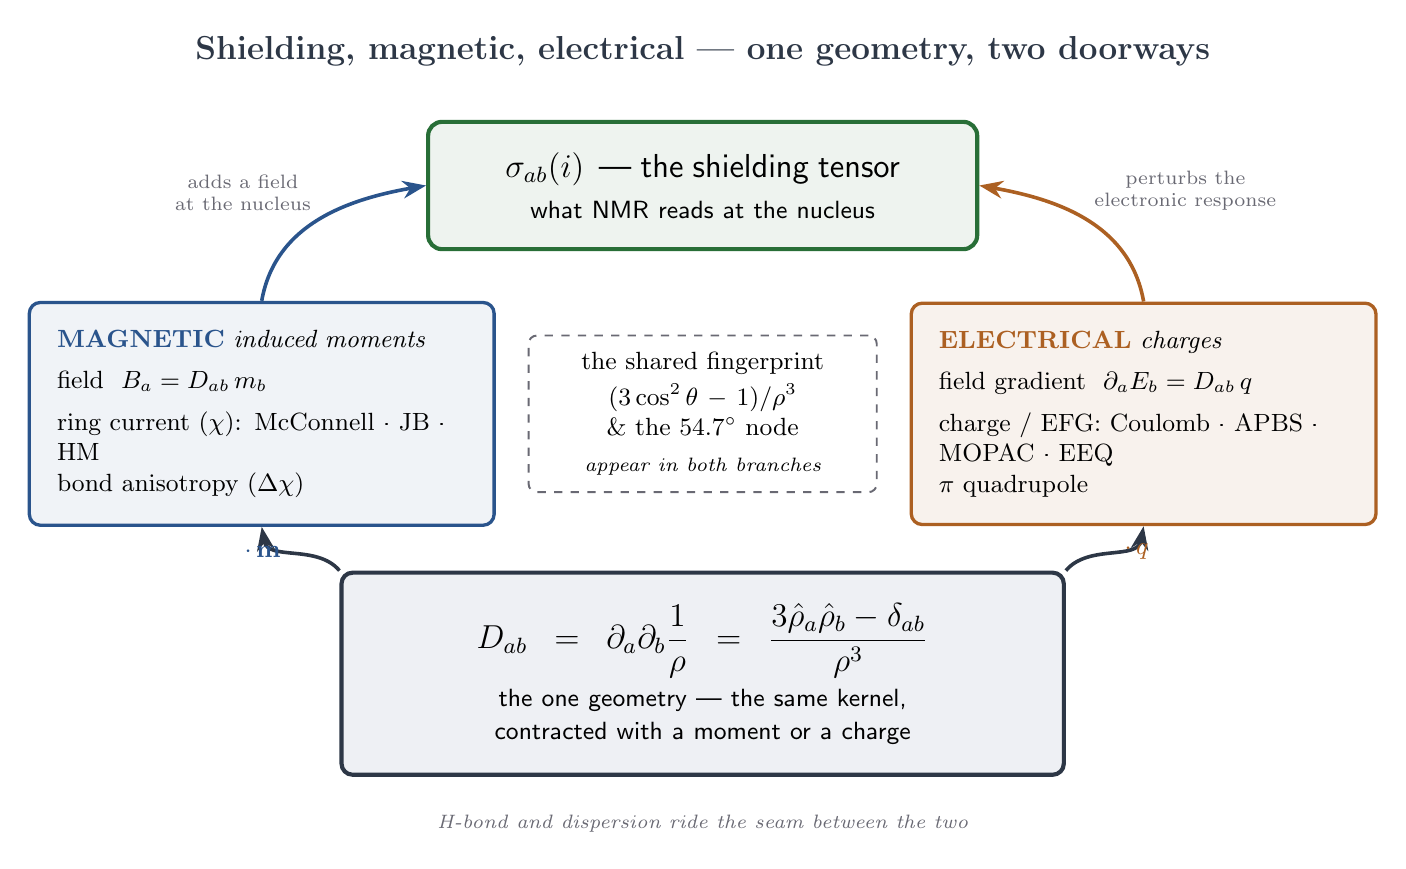
\begin{tikzpicture}[
  font=\sffamily,
  >={Stealth[length=3mm]},
  obs/.style={rounded corners=5pt, draw=tObs, line width=1.5pt, fill=tObs!8, align=center, inner sep=11pt, text width=6.2cm},
  mag/.style={rounded corners=4pt, draw=tMag, line width=1.2pt, fill=tMag!7, align=left, inner sep=10pt, text width=5.2cm, font=\small},
  elec/.style={rounded corners=4pt, draw=tElec, line width=1.2pt, fill=tElec!8, align=left, inner sep=10pt, text width=5.2cm, font=\small},
  ker/.style={rounded corners=4pt, draw=ink, line width=1.5pt, fill=cLaw, align=center, inner sep=11pt, text width=8.4cm},
]

% ---- title ----
\node[font=\large\bfseries, text=ink] (T) at (0,5.9) {Shielding, magnetic, electrical --- one geometry, two doorways};

% ---- the observable (apex) ----
\node[obs] (OBS) at (0,4.2) {%
  {\large $\sigma_{ab}(i)$\, --- the shielding tensor}\\[3pt]
  {\small what NMR reads at the nucleus}};

% ---- the two faces ----
\node[mag] (MAG) at (-5.6,1.3) {%
  {\bfseries\textcolor{tMag}{MAGNETIC}}\ {\small\itshape induced moments}\\[4pt]
  field\ \ $B_a = D_{ab}\,m_b$\\[4pt]
  {\small ring current ($\chi$): McConnell \textperiodcentered\ JB \textperiodcentered\ HM}\\
  {\small bond anisotropy ($\Delta\chi$)}};

\node[elec] (ELEC) at (5.6,1.3) {%
  {\bfseries\textcolor{tElec}{ELECTRICAL}}\ {\small\itshape charges}\\[4pt]
  field gradient\ \ $\partial_a E_b = D_{ab}\,q$\\[4pt]
  {\small charge / EFG: Coulomb \textperiodcentered\ APBS \textperiodcentered\ MOPAC \textperiodcentered\ EEQ}\\
  {\small $\pi$ quadrupole}};

% ---- the shared root ----
\node[ker] (KER) at (0,-2.0) {%
  {\large $\displaystyle D_{ab}=\partial_a\partial_b\frac{1}{\rho}=\frac{3\hat\rho_a\hat\rho_b-\delta_{ab}}{\rho^{3}}$}\\[3pt]
  {\small the one geometry --- the same kernel, contracted with a moment or a charge}};

% ---- fork: kernel -> faces ----
\draw[->, line width=1.3pt, ink] (KER.north west) to[out=130,in=-80]
   node[midway, left=1pt, font=\small, text=tMag] {$\cdot\,\mathbf m$} (MAG.south);
\draw[->, line width=1.3pt, ink] (KER.north east) to[out=50,in=-100]
   node[midway, right=1pt, font=\small, text=tElec] {$\cdot\,q$} (ELEC.south);

% ---- funnel: faces -> observable ----
\draw[->, line width=1.3pt, tMag] (MAG.north) to[out=80,in=190]
   node[midway, above left=-1pt, font=\scriptsize, text=note, align=center] {adds a field\\ at the nucleus} (OBS.west);
\draw[->, line width=1.3pt, tElec] (ELEC.north) to[out=100,in=-10]
   node[midway, above right=-1pt, font=\scriptsize, text=note, align=center] {perturbs the\\ electronic response} (OBS.east);

% ---- the shared fingerprint (between the faces) ----
\node[rounded corners=3pt, draw=note, dashed, line width=0.7pt, fill=white, align=center,
      inner sep=6pt, text width=4.0cm, font=\small] (FP) at (0,1.3) {%
  the shared fingerprint\\[2pt]
  $(3\cos^2\theta-1)/\rho^3$\ \ \&\ the $54.7^\circ$ node\\[2pt]
  {\scriptsize\itshape appear in both branches}};

% ---- the seam ----
\node[font=\scriptsize\itshape, text=note] at (0,-3.9) {H-bond and dispersion ride the seam between the two};

\end{tikzpicture}
\end{document}
